\chapter{Måling på volumenkontrol}
\label{maalevolumenkontrol}

Denne målerapport dokumenterer målinger foretaget på projektets volumenkontrol, opbygget som beskrevet i kapitel \ref{volumenkontrol}. Målingerne er foretaget på Fredrik Bajers Vej 7 i lokale B1-104 på Aalborg Universitet den 17. december 2010 af gruppe 311.

\subsection*{Formål}
Målingernes formål er at teste:
\begin{itemize}
\item Brugerfladefunktionen
\item Funktionen
\end{itemize}

\subsection*{Testobjekt}


\subsection*{Måleopstilling}


\subsection*{Anvendt udstyr}

\begin{table}[h]
\centering
\begin{tabular}{l|c|l}
\hline\hline
Instrument & AAU-nr. & Fabrikant, type m.v. \\
\hline\hline
Oscilloskop & 33857 & Agilent 54621A \\[4pt]
Oscillator & 07995 & B\&O RC-oscillator TG7 \\[4pt]
Spændingsforsyning & 33908 & HAMEG HM7042 \\[4pt]
Spændingsforsyning & 33907 & HAMEG HM7042 \\[4pt]
Audioanalysator & 76986 & National Instruments NI-PCI-4461 \\
\hline\hline
\end{tabular}
\label{tab:maaleudstyr_forforstaerker}
\end{table}

\subsection*{Måleprocedure}
Proceduren for målingen er:

\begin{enumerate}
\item Generatoren indstilles til en peak-peakspænding på 4.41 V (indstilles med oscilloskop) ved 1 kHz og tilsluttes
\item Den ene spændingsforsyning indstilles til 5 V og tilsluttes kontrollogikken
\item Den anden spændingsforsyning indstilles til $\pm$15 V og tilsluttes dæmperen
\item Alle trin gennemløbes hvor generatorspændingen og output noteres
\item Alle trin gennemløbes med nedholdt knap og displayvisningen observeres
\end{enumerate}

\subsection*{Resultater}

Resultaterne for målingen af dæmpningen kan aflæses i tabel \ref{tab:resultat_volumenkontrol} og \ref{tab:resultat_volumenkontrol2}.

\begin{table}[h]
\begin{minipage}[b]{0.45\linewidth}
\centering
\begin{tabular}{l|c|l}
\hline\hline
Displaytrin & Peak-peak output & Enhed \\
\hline\hline
0 dB & 4,81 & V \\[4pt]
1 dB & 4,25 & V \\[4pt]
2 dB & 3,85 & V \\[4pt]
3 dB & 3,44 & V \\[4pt]
4 dB & 3,03 & V \\[4pt]
5 dB & 2,75 & V \\[4pt]
6 dB & 2,47 & V \\[4pt]
7 dB & 2,22 & V \\[4pt]
8 dB & 1,78 & V \\[4pt]
9 dB & 1,50 & V \\[4pt]
10 dB & 1,35 & V \\[4pt]
11 dB & 1,2 & V \\[4pt]
12 dB & 1 & V \\[4pt]
13 dB & 950 & mV \\[4pt]
14 dB & 838 & mV \\[4pt]
15 dB & 750 & mV \\[4pt]
16 dB & 750 & mV \\[4pt]
17 dB & 672 & mV \\[4pt]
18 dB & 603 & mV \\[4pt]
19 dB & 537 & mV \\[4pt]
20 dB & 478 & mV \\[4pt]
21 dB & 431 & mV \\[4pt]
22 dB & 384 & mV \\[4pt]
23 dB & 330 & mV \\[4pt]
24 dB & 303 & mV \\[4pt]
25 dB & 273 & mV \\
\hline\hline
\end{tabular}
\caption{Resultater fra 0 til 25 dB af måling}
\label{tab:resultat_volumenkontrol}
\end{minipage}
\hspace{0.5cm}
\begin{minipage}[b]{0.45\linewidth}
\begin{tabular}{l|c|l}
\hline\hline
Displaytrin & Peak-peak output & Enhed \\
\hline\hline
26 dB & 244 & mV \\[4pt]
27 dB & 216 & mV \\[4pt]
28 dB & 197 & mV \\[4pt]
29 dB & 177 & mV \\[4pt]
30 dB & 156 & mV \\[4pt]
31 dB & 140 & mV \\[4pt]
32 dB & 127 & mV \\[4pt]
33 dB & 108 & mV \\[4pt]
34 dB & 100 & mV \\[4pt]
35 dB & 87 & mV \\[4pt]
36 dB & 78 & mV \\[4pt]
37 dB & 70 & mV \\[4pt]
38 dB & 62 & mV \\[4pt]
39 dB & 58 & mV \\[4pt]
40 dB & 51 & mV \\[4pt]
41 dB & 45 & mV \\[4pt]
42 dB & 40 & mV \\[4pt]
43 dB & 36 & mV \\[4pt]
44 dB & 33 & mV \\[4pt]
45 dB & 30 & mV \\[4pt]
46 dB & 27 & mV \\[4pt]
47 dB & 24 & mV \\[4pt]
48 dB & 21 & mV \\[4pt]
49 dB & 19 & mV \\[4pt]
50 dB & 18 & mV \\
& & \\[4pt]
\hline\hline
\end{tabular}
\caption{Resultater fra 26 til 50 dB af måling}
\label{tab:resultat_volumenkontrol2}
\end{minipage}
\end{table}

THD målingen og frekvensgangen er målt ved 200 mV og 2 V peakspænding. Da disse er meget ens, vises kun den ene, 2 V, da det er denne der har de største værdier. Resultaterne er vist på figur \ref{fig:apvold:frek0} til \ref{fig:apvold:thd50}

\begin{figure}[h]
\centering
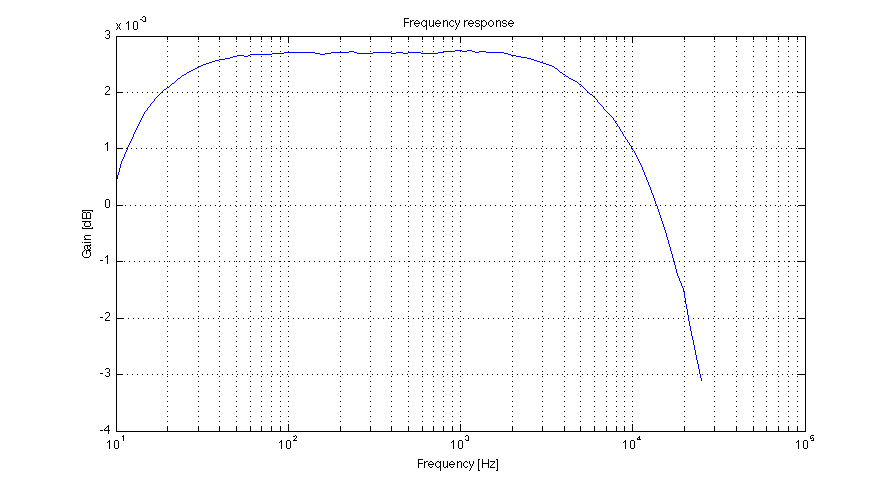
\includegraphics[width=\textwidth]{maalerapporter/volumenkontrol/2Vniveau0-frek.png}
\caption{Frekvensgang for volumenkontrollen ved fuldt signal}
\label{fig:apvold:frek0}
\end{figure}

\begin{figure}[h]
\centering
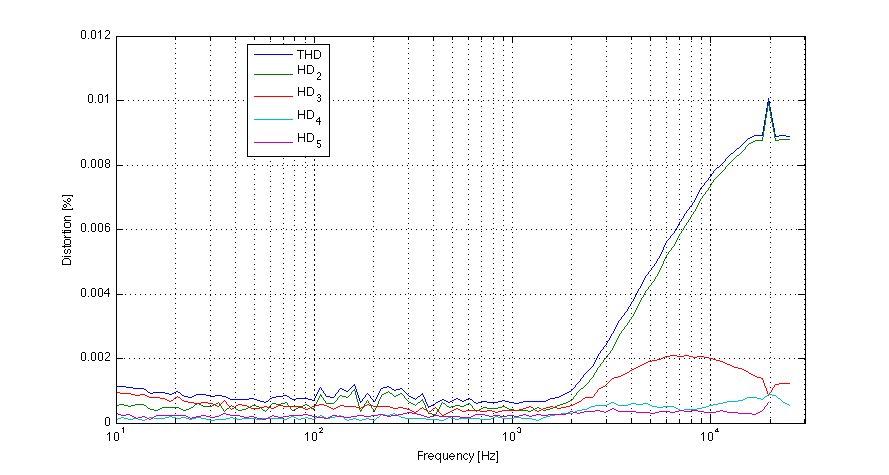
\includegraphics[width=\textwidth]{maalerapporter/volumenkontrol/2Vniveau0-thd.png}
\caption{THD for volumenkontrollen ved fuldt signal}
\end{figure}

\begin{figure}[h]
\centering
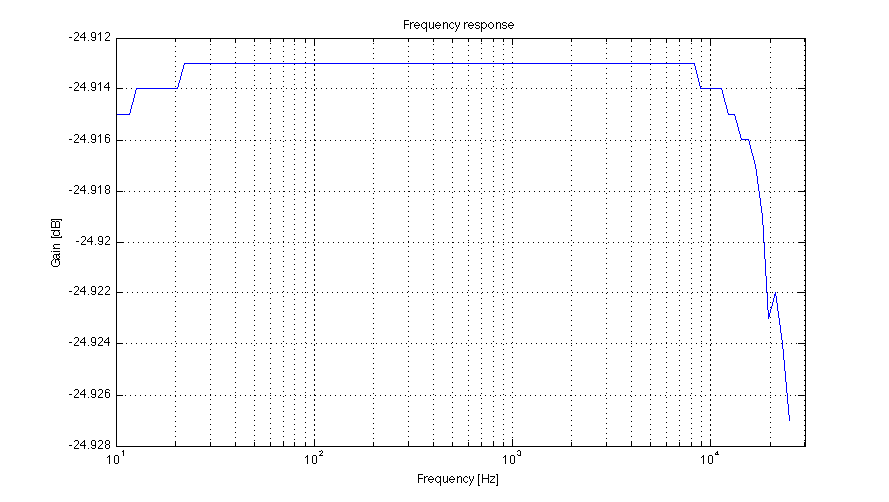
\includegraphics[width=\textwidth]{maalerapporter/volumenkontrol/2Vniveau25-frek.png}
\caption{Frekvensgang for volumenkontrollen ved 25 dB's dæmpning}
\end{figure}

\begin{figure}[h]
\centering
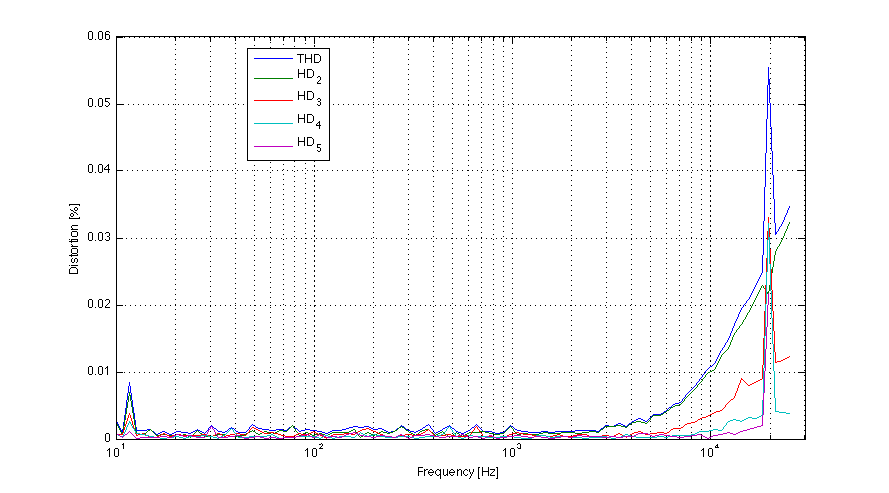
\includegraphics[width=\textwidth]{maalerapporter/volumenkontrol/2Vniveau25-thd.png}
\caption{THD for volumenkontrollen ved 25 dB's dæmpning}
\end{figure}

\begin{figure}[h]
\centering
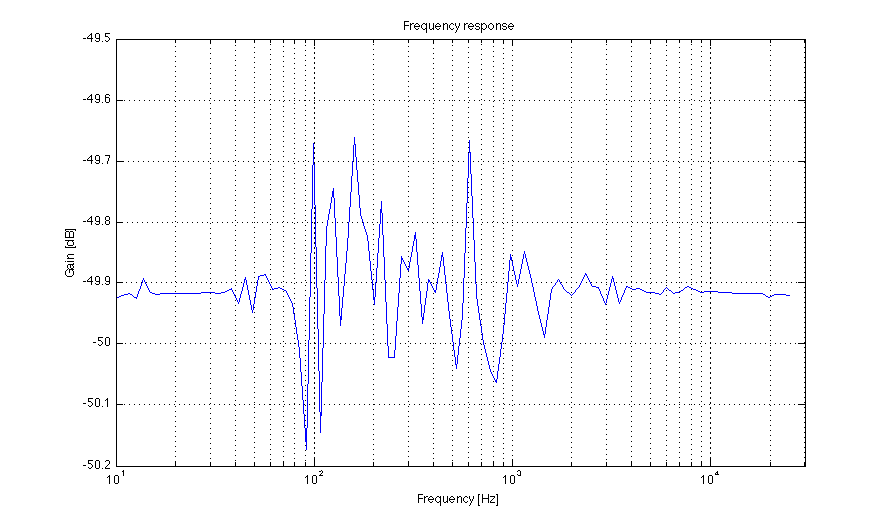
\includegraphics[width=\textwidth]{maalerapporter/volumenkontrol/2Vniveau50-frek.png}
\caption{Frekvensgang for volumenkontrollen ved 50 dB's dæmpning}
\end{figure}

\begin{figure}[h]
\centering
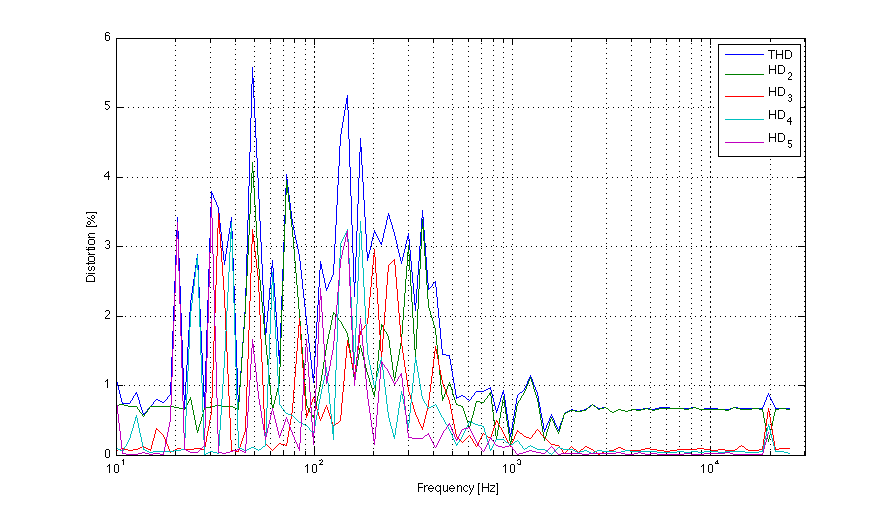
\includegraphics[width=\textwidth]{maalerapporter/volumenkontrol/2Vniveau50-thd.png}
\caption{THD for volumenkontrollen ved 50 dB's dæmpning}
\label{fig:apvold:thd50}
\end{figure}

Volumenkontrollen er observeret til ikke altid at gøre som det var tilsigtet. Responset fra knapperne giver ikke altid den tilsigtede ændring i dæmpning og den øvre grænser er 51. Accelerationen virker som tilsigtet.

\subsection*{Måleusikkerheder}
I forbindelse med målingerne er der naturligt en række usikkerheder som kan spille ind på resultaterne. Disse usikkerheder vil ikke her blive vurderet på. 

\begin{itemize}
\item Aflæsningsunøjagtigheder
\item Udstyrstolerancer
\item Måleinstrumenter belaster måleobjektet
\end{itemize}